\section{Experiments}
\label{sec:experiments}

\begin{table}[t]
  \centering
  \caption{Video accuracy (\%) of the four fusion variants on the original
  (leaky) and corrected splits. $\Delta$: test-accuracy change in pp when
  identity leakage is removed. Video models are warm-started from the
  per-frame model of the same split.}
  \label{tab:fusion}
  \setlength{\tabcolsep}{4pt}
  \begin{tabular}{lrrrrrr}
    \toprule
    & & \multicolumn{2}{c}{Original} & \multicolumn{2}{c}{Corrected} & \\
    \cmidrule(lr){3-4}\cmidrule(lr){5-6}
    Model & Params & Val & Test & Val & Test & $\Delta$ \\
    \midrule
    Per-frame    & 2.33\,M & 93.3 & 91.7 & 40.8 & 35.0 & $-$56.7 \\
    Late fusion  & 2.33\,M & 93.3 & 93.3 & 43.3 & 38.3 & $-$55.0 \\
    Early fusion & 2.35\,M & 89.2 & 91.7 & 40.0 & 36.7 & $-$55.0 \\
    3D CNN       & 6.98\,M & 92.5 & 90.8 & 34.2 & 41.7 & $-$49.2 \\
    \bottomrule
  \end{tabular}
\end{table}

\begin{table}[t]
  \centering
  \caption{Two-stream results on the corrected splits (video accuracy, \%).
  The fusion weight $w$ is selected on validation only; equal weighting
  ($w=0.5$) gives the same accuracies.}
  \label{tab:twostream}
  \begin{tabular}{lrr}
    \toprule
    Model & Val & Test \\
    \midrule
    RGB stream (late fusion)                 & 43.3 & 38.3 \\
    Flow stream (stacked flow)               & 55.8 & 49.2 \\
    Score fusion, $w=0.55$ (val.-selected)   & 58.3 & 54.2 \\
    Joint dual stream                        & 55.0 & 54.2 \\
    \bottomrule
  \end{tabular}
\end{table}

\begin{figure*}[t]
  \centering
  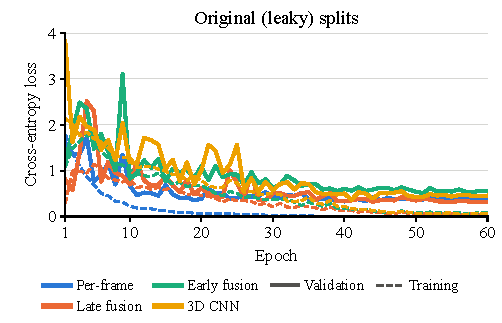
\includegraphics[width=0.49\textwidth]{figures/v2_loss_original.pdf}\hfill
  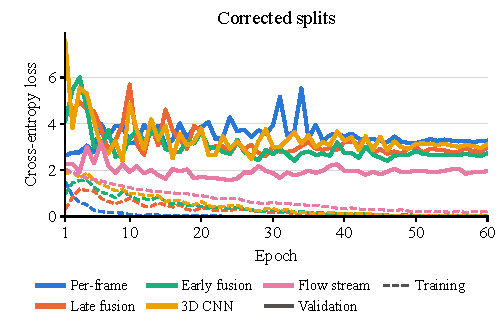
\includegraphics[width=0.49\textwidth]{figures/v2_loss_corrected.pdf}
  \caption{Training (dashed) and validation (solid) cross-entropy loss per
  epoch on the original (left) and corrected (right) splits, seed 42.
  Per-frame training loss is computed on single frames; all validation
  losses are video-level.}
  \label{fig:curves}
\end{figure*}

\subsection{Where to fuse time (Task 4.1)}
On the original splits all four variants reach 89--93\% validation and
91--93\% test accuracy (\cref{tab:fusion}). The largest test gap, late fusion
against the 3D CNN, is three videos (2.5\,pp), which is about one binomial
standard error at this accuracy. No fusion point is therefore clearly better,
matching Karpathy \etal's observation that single-frame models are hard to
beat~\cite{karpathy2014largescale}. Early fusion and the 3D CNN now fit the
training set (98\% final training accuracy, \cref{fig:curves}, left),
passing the check that the first backbone failed.

\subsection{Information leakage (Task 4.2.1)}
Because the original splits share people and settings across splits, a
model can score well by recognising them instead of the action. Retrained with the same recipe on the corrected splits, every RGB model loses
49--57\,pp of test accuracy, falling to 35--42\%, while its training
accuracy still reaches ${\geq}99\%$ and its validation loss stays near 3
(\cref{fig:curves}, right). The models had
memorised people and settings. Their ranking is not stable: the 3D CNN is
the weakest on validation (34.2\%) but the strongest on test (41.7\%), where
it drops the least. With a standard error of about 4.5\,pp at 40\% accuracy,
the four RGB variants remain indistinguishable on the corrected splits.

\subsection{Optical flow (Task 4.2.2)}
The flow stream alone reaches 55.8\% validation and 49.2\% test accuracy,
12.5 and 10.8\,pp above the RGB stream, and it fits the training set more
slowly (83\% at its selected epoch). Motion therefore transfers across
people far better than appearance. Score fusion adds a further 2.5\,pp on
validation and 5.0\,pp on test (54.2\%), because the streams fail on
different classes. On test, flow recognises JumpingJack (11/12 videos,
against 5/12 for RGB), BodyWeightSquats (8 against 1), and PushUps
(8 against 4), whereas RGB identifies TrampolineJumping from its scene
(10 against 2). Fusion only helps once $w\geq0.3$: below that, the
overfitted, overconfident RGB stream (validation NLL 2.91, against 1.86 for
flow) dominates the average. Joint training matches score fusion on test
(54.2\%) but is 3.3\,pp lower on validation (55.0\%), so neither way of
combining the streams is clearly better.
